\documentclass{article}

\usepackage{arxiv}

\usepackage[utf8]{inputenc}
\usepackage[T1]{fontenc}
\usepackage{hyperref}
\usepackage{url}
\usepackage{booktabs}
\usepackage{amsfonts}
\usepackage{amsmath}
\usepackage{amssymb}
\usepackage{nicefrac}
\usepackage{microtype}
\usepackage{graphicx}
\usepackage{multirow}
\usepackage{natbib}
\usepackage{doi}
\usepackage{xcolor}
\usepackage{tikz}
\usetikzlibrary{arrows.meta, positioning, shapes.geometric, calc, decorations.pathmorphing, fit, backgrounds}
\usepackage{multirow}
\usepackage{enumitem}
\usepackage{caption}
\usepackage{subcaption}

% Custom marks for comparison table
\newcommand{\fullmark}{\checkmark}
\newcommand{\halfmark}{$\sim$}

\hypersetup{
  colorlinks=true,
  linkcolor=blue!70!black,
  citecolor=green!50!black,
  urlcolor=blue!60!black,
  pdftitle={The Knowledge Lifecycle of Large Language Models},
  pdfsubject={cs.CL},
  pdfauthor={Amey Thakur},
  pdfkeywords={Large Language Models, Knowledge Lifecycle, RAG, Knowledge Editing, Continual Learning, Machine Unlearning},
}

\title{The Knowledge Lifecycle of Large Language Models}

\author{
	\href{https://orcid.org/0000-0001-5644-1575}{
\includegraphics[scale=0.06]{orcid.png}\hspace{1mm}Amey Thakur} \\
	Independent Researcher \\
	Toronto, Canada \\
	\texttt{ameythakur20@gmail.com} \\
}

\renewcommand{\undertitle}{}
\renewcommand{\headeright}{}
\renewcommand{\shorttitle}{The Knowledge Lifecycle of LLMs}

\begin{document}
\maketitle

\begin{abstract}
Five distinct research communities now study how large language models handle knowledge: retrieval-augmented generation, knowledge editing, continual learning, context engineering, and agent memory. These communities publish in different venues, use different evaluation protocols, and rarely cite one another. The result is a fragmented understanding of a single underlying problem. This survey introduces the \textbf{Knowledge Lifecycle}, a framework that organises the full span of LLM knowledge research into five stages: \textit{Acquisition}, \textit{Storage}, \textit{Retrieval}, \textit{Update}, and \textit{Forgetting}. Drawing on over 150 primary sources, we trace each stage in detail and, more importantly, expose the failure modes that arise at the boundaries between stages (for example, when edited parametric knowledge contradicts retrieved external knowledge). We close with concrete open problems that no single-stage survey can identify. Our central claim is that progress on knowledge in LLMs requires thinking in terms of lifecycles, not isolated components.
\end{abstract}

% ============================================================
\section{Introduction}
\label{sec:introduction}
% ============================================================

Large language models now serve as the backbone of systems that answer medical questions, draft legal briefs, write production code, and tutor students in mathematics~\citep{brown2020language, achiam2023gpt4, team2023gemini}. All of these applications depend, in one way or another, on the model's relationship with knowledge. A medical assistant that cites a retracted drug interaction, a coding agent that cannot incorporate an updated API, or a chatbot that leaks a user's deleted personal data all represent failures of knowledge management, not failures of language modelling.

The research community has responded to these challenges, but it has done so in silos. General surveys on LLMs~\citep{zhao2023llm_survey, wang2024llm_agents_survey} touch on knowledge tangentially, while specific subfields operate in isolation. At least five separate subfields now address different pieces of the knowledge problem:

\begin{enumerate}[leftmargin=*]
  \item \textbf{Retrieval-Augmented Generation (RAG)} focuses on how to fetch relevant documents and feed them to the model at inference time~\citep{lewis2020rag, guu2020realm, gao2023rag_survey}.
  \item \textbf{Knowledge Editing} asks whether individual facts inside a model's weights can be surgically modified without retraining~\citep{meng2022locating, meng2023memit, yao2023editing_survey}.
  \item \textbf{Continual Learning} tackles how a model can absorb new information over time without destroying what it already knows~\citep{kirkpatrick2017ewc, ke2023continual, wu2024continual_survey}.
  \item \textbf{Context Engineering} studies how to arrange, compress, and prioritise information within a finite context window~\citep{liu2024lost}.
  \item \textbf{Agent Memory} builds persistent storage that lets LLM-based agents remember and reuse past experience~\citep{park2023generative, packer2023memgpt, zhang2024survey_agent_memory}.
\end{enumerate}

Each subfield has its own dedicated surveys~\citep{gao2023rag_survey, mialon2023augmented, zhang2024survey_agent_memory, wang2024human_to_ai_memory}. None of them talks to the others in a structured way. A researcher improving a RAG retriever seldom considers what happens when retrieved facts contradict the model's parametric memory. A team building a knowledge editor rarely checks whether their edits survive continual fine-tuning. These blind spots are not academic curiosities; they cause real system failures.

This survey takes a different approach. We treat all five subfields as stages of a single process: the \textbf{Knowledge Lifecycle} of large language models. The lifecycle has five stages: how knowledge is \textit{acquired} (\S\ref{sec:acquisition}), where it is \textit{stored} (\S\ref{sec:storage}), how it is \textit{retrieved} when needed (\S\ref{sec:retrieval}), how it is \textit{updated} as the world changes (\S\ref{sec:update}), and how it is \textit{forgotten}, whether deliberately or by accident (\S\ref{sec:forgetting}).

\paragraph{Contributions.} We make three contributions:

\begin{enumerate}[leftmargin=*]
  \item \textbf{A lifecycle framework} that maps existing research across five stages. For each stage, we review the primary methods, trace their intellectual origins, and pin down the assumptions they rely on.

  \item \textbf{Cross-stage analysis} (\S\ref{sec:analysis}). We identify failure modes that only become visible when two stages interact. For instance, knowledge editing can succeed locally yet create inconsistencies that surface during retrieval. Continual learning can acquire new knowledge while silently degrading unrelated facts. These boundary failures cannot be diagnosed by any single-stage benchmark.

  \item \textbf{Open problems} (\S\ref{sec:open_problems}) that arise specifically from the lifecycle view: the absence of end-to-end benchmarks, the need for knowledge provenance tracking, and the challenge of maintaining consistency across parametric and non-parametric stores.
\end{enumerate}

We draw on over 150 papers from NeurIPS, ICML, ACL, EMNLP, ICLR, Nature, and JMLR published between 2014 and 2026. To our knowledge, no prior survey covers all five lifecycle stages within a single framework.

% ============================================================
\section{Background and Scope}
\label{sec:background}
% ============================================================

\subsection{What Counts as ``Knowledge'' in an LLM?}

We use ``knowledge'' broadly. For the purposes of this survey, knowledge is any information, whether factual, procedural, or experiential, that shapes a model's outputs. Four varieties matter here:

\begin{itemize}[leftmargin=*]
  \item \textbf{Factual knowledge.} Concrete facts about the world (``The boiling point of water at sea level is 100\textdegree C''), acquired mainly during pre-training~\citep{petroni2019lama}.
  \item \textbf{Procedural knowledge.} How to carry out tasks: following multi-step instructions, writing code in a particular style, or reasoning through a chain of logic. This is typically instilled through instruction tuning and RLHF~\citep{ouyang2022instructgpt, wei2022finetuned}.
  \item \textbf{Experiential knowledge.} Records of past interactions, user preferences, and task outcomes kept by agent memory systems~\citep{park2023generative, packer2023memgpt}.
  \item \textbf{Contextual knowledge.} Information provided at inference time via the prompt or fetched from an external source~\citep{lewis2020rag}.
\end{itemize}

One important observation: the same fact can exist in multiple forms simultaneously. ``The CEO of OpenAI is Sam Altman'' might live in the model's weights (parametric), in a vector database (non-parametric), and in the current prompt (contextual). Each copy follows a different lifecycle path, with different update and deletion properties.

\subsection{Positioning Among Existing Surveys}

Table~\ref{tab:survey_comparison} shows where prior surveys sit. Each one covers one or two lifecycle stages in depth; none attempts the full picture. The table makes the gap concrete.

\begin{table}[t]
\centering
\caption{Coverage of lifecycle stages by existing surveys. \fullmark\ = primary focus; \halfmark\ = partial; -- = absent.}
\label{tab:survey_comparison}
\small
\begin{tabular}{@{}lccccc@{}}
\toprule
\textbf{Survey} & \textbf{Acquire} & \textbf{Store} & \textbf{Retrieve} & \textbf{Update} & \textbf{Forget} \\
\midrule
Gao et al.\ (2023), RAG Survey & -- & \halfmark & \fullmark & -- & -- \\
Mialon et al.\ (2023), Augmented LMs & \halfmark & -- & \fullmark & -- & -- \\
Yao et al.\ (2023), Knowledge Editing & -- & \halfmark & -- & \fullmark & -- \\
Wu et al.\ (2024), Continual Learning & \halfmark & -- & -- & \fullmark & \halfmark \\
Zhang et al.\ (2025), Agent Memory & -- & \fullmark & \fullmark & \halfmark & \halfmark \\
Wang et al.\ (2025), Human$\to$AI Memory & \halfmark & \fullmark & \halfmark & \halfmark & -- \\
\midrule
\textbf{This survey} & \fullmark & \fullmark & \fullmark & \fullmark & \fullmark \\
\bottomrule
\end{tabular}
\vspace{-1em}
\end{table}

\subsection{Scope and Boundaries}

We restrict attention to text-based LLMs built on the Transformer architecture~\citep{vaswani2017attention}. Multimodal extensions (images, video, audio) appear only in our discussion of future work (\S\ref{sec:open_problems}). When we discuss agent memory, we treat the LLM as a component inside a larger agent system and make the boundary explicit.

% ============================================================
\section{The Knowledge Lifecycle Framework}
\label{sec:framework}
% ============================================================

The lifecycle has five stages. Each one maps to a well-defined set of research questions. Figure~\ref{fig:lifecycle} gives the visual overview.

\begin{figure*}[t]
\centering
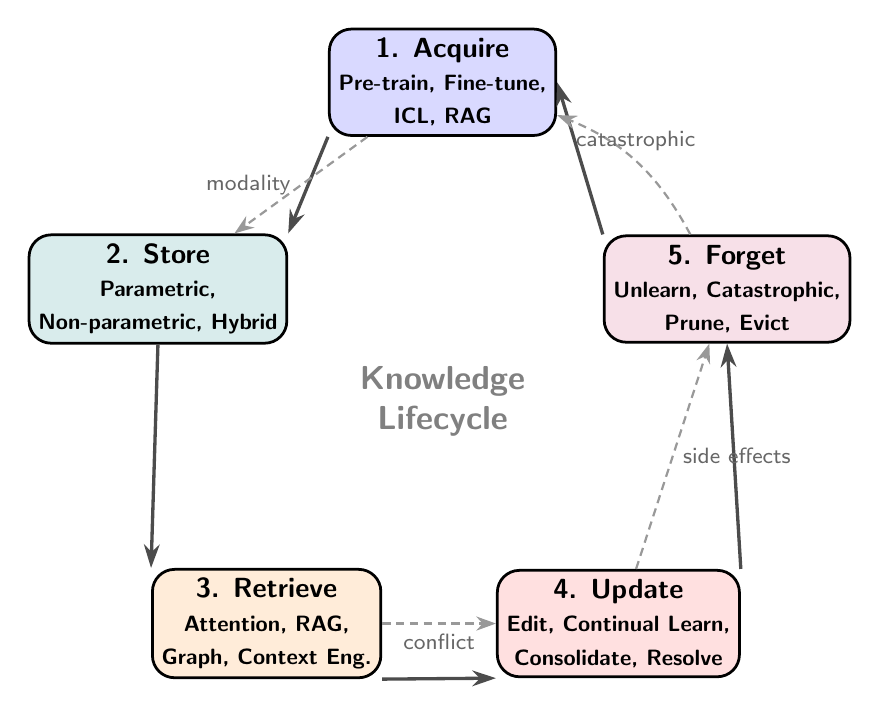
\begin{tikzpicture}[
  stage/.style={
    draw, rounded corners=8pt, minimum width=2.6cm, minimum height=1.2cm,
    font=\sffamily\bfseries, align=center, line width=1pt
  },
  arrow/.style={-{Stealth[length=3mm,width=2mm]}, line width=1.2pt, color=black!70},
  backarrow/.style={-{Stealth[length=2.5mm,width=1.8mm]}, line width=0.8pt, densely dashed, color=black!40},
  note/.style={font=\sffamily\footnotesize, text=black!60, align=center}
]

% --- Five stages arranged in a pentagon ---
\def\R{3.8}
\node[stage, fill=blue!15] (acq) at (90:\R) {\textbf{1. Acquire}\\{\footnotesize Pre-train, Fine-tune,}\\{\footnotesize ICL, RAG}};
\node[stage, fill=teal!15] (sto) at (162:\R) {\textbf{2. Store}\\{\footnotesize Parametric,}\\{\footnotesize Non-parametric, Hybrid}};
\node[stage, fill=orange!15] (ret) at (234:\R) {\textbf{3. Retrieve}\\{\footnotesize Attention, RAG,}\\{\footnotesize Graph, Context Eng.}};
\node[stage, fill=red!12] (upd) at (306:\R) {\textbf{4. Update}\\{\footnotesize Edit, Continual Learn,}\\{\footnotesize Consolidate, Resolve}};
\node[stage, fill=purple!12] (fgt) at (18:\R) {\textbf{5. Forget}\\{\footnotesize Unlearn, Catastrophic,}\\{\footnotesize Prune, Evict}};

% --- Forward arrows (main lifecycle flow) ---
\draw[arrow] (acq.south west) -- (sto.north east);
\draw[arrow] (sto.south) -- (ret.north west);
\draw[arrow] (ret.south east) -- (upd.south west);
\draw[arrow] (upd.north east) -- (fgt.south);
\draw[arrow] (fgt.north west) -- (acq.east);

% --- Cross-stage interaction arrows (dashed) ---
\draw[backarrow] (ret) -- (upd) node[midway, below, note] {conflict};
\draw[backarrow] (upd) -- (fgt) node[midway, right, note] {side effects};
\draw[backarrow] (fgt) to[bend right=20] node[midway, above, note] {catastrophic} (acq);
\draw[backarrow] (acq) -- (sto) node[midway, left, note] {modality};

% --- Centre label ---
\node[font=\sffamily\large\bfseries, text=black!50] at (0,0) {Knowledge};
\node[font=\sffamily\large\bfseries, text=black!50] at (0,-0.5) {Lifecycle};

\end{tikzpicture}
\caption{The Knowledge Lifecycle framework. Solid arrows show the primary flow of knowledge through five stages. Dashed arrows indicate cross-stage interactions that produce failure modes (knowledge conflicts, catastrophic forgetting, unintended side effects). Each stage maps to a distinct body of research, but the interactions between stages are where the hardest open problems lie.}
\label{fig:lifecycle}
\end{figure*}

\subsection{Overview of the Five Stages}

\paragraph{Stage 1: Acquisition.} Knowledge enters the system. Pre-training compresses billions of web pages into parameters. Fine-tuning injects specialised task or domain knowledge. In-context learning supplies knowledge transiently through demonstrations placed in the prompt. Retrieval-augmented pre-training (REALM~\citep{guu2020realm}, Atlas~\citep{izacard2022atlas}) teaches the model to pull in external text during training itself.

\paragraph{Stage 2: Storage.} Acquired knowledge has to live somewhere. We identify four storage modalities: \textit{parametric} (baked into weights), \textit{non-parametric} (sitting in a vector database, knowledge graph, or document index), \textit{hybrid} (architectures such as RETRO~\citep{borgeaud2022retro} that blend both), and \textit{agent memory hierarchies} (tiered systems with working, episodic, and archival layers~\citep{packer2023memgpt}).

\paragraph{Stage 3: Retrieval.} A question arrives. The system must locate the right knowledge and bring it to bear. Internal retrieval works through the self-attention mechanism. External retrieval is the RAG pipeline: encode the query, search the index, return the top passages. Context engineering (choosing which passages to include, in what order, and in what format) determines whether retrieved knowledge actually reaches the model's reasoning process.

\paragraph{Stage 4: Update.} The world changes, and the system's knowledge must change with it. Knowledge editing rewrites individual facts in the weights~\citep{meng2022locating, meng2023memit}. Continual learning extends the model to new domains over time~\citep{kirkpatrick2017ewc}. Agent memory consolidation turns raw interaction logs into distilled insights~\citep{park2023generative}. Knowledge conflict resolution decides what to do when the weights say one thing and the retrieved document says another~\citep{xie2024knowledge_conflicts}.

\paragraph{Stage 5: Forgetting.} Knowledge leaves the system, on purpose or by accident. Machine unlearning removes specific facts to comply with privacy law~\citep{jang2023unlearning, maini2024tofu}. Catastrophic forgetting destroys old knowledge as a side effect of learning new knowledge~\citep{kirkpatrick2017ewc, luo2024empirical_catastrophic}. Selective pruning trims bloated agent memory stores. KV-cache eviction drops tokens that no longer fit in the context window.

\subsection{Cross-Stage Dependencies}

The five stages are not a linear pipeline. They interact, and those interactions create problems that no single stage can solve alone:

\begin{itemize}[leftmargin=*]
  \item \textbf{Acquisition $\leftrightarrow$ Storage.} How knowledge is acquired dictates where it ends up. Pre-training stores knowledge parametrically; RAG stores it externally. This choice echoes through every later stage.
  \item \textbf{Storage $\leftrightarrow$ Retrieval.} Parametric storage relies on implicit retrieval through attention. Non-parametric storage requires an explicit search pipeline. The retrieval mechanism must match the storage format.
  \item \textbf{Retrieval $\leftrightarrow$ Update.} Editing a fact in the weights does not edit it in the vector database, and vice versa. When the two copies disagree, the system produces contradictory outputs.
  \item \textbf{Update $\leftrightarrow$ Forgetting.} Every edit is a small forgetting event (the old fact is overwritten). Every unlearning operation risks collateral damage to neighbouring facts. The two problems share root causes.
  \item \textbf{Forgetting $\leftrightarrow$ Acquisition.} Catastrophic forgetting during continual training and deliberate unlearning for privacy are studied by different communities, but both boil down to the same question: how to selectively remove information from entangled representations.
\end{itemize}

We return to these interactions in \S\ref{sec:analysis}. The next five sections examine each stage in turn.

% ============================================================
\section{Acquisition: How LLMs Gain Knowledge}
\label{sec:acquisition}
% ============================================================

\begin{figure*}[t]
\centering
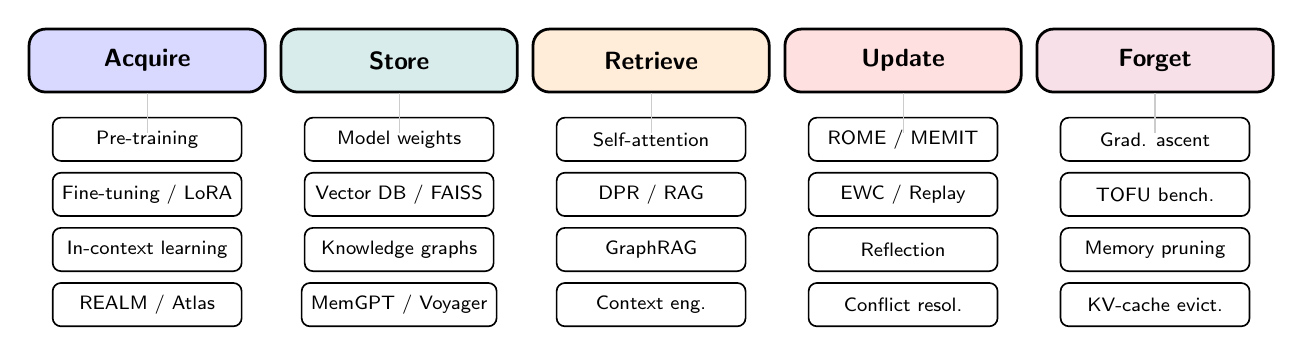
\begin{tikzpicture}[
  stageheader/.style={draw, rounded corners=6pt, minimum width=3cm, minimum height=0.8cm, font=\sffamily\bfseries\small, align=center, line width=1pt},
  method/.style={draw, rounded corners=3pt, minimum width=2.4cm, minimum height=0.55cm, font=\sffamily\scriptsize, align=center, line width=0.6pt, fill=white},
  groupbox/.style={draw, rounded corners=6pt, dashed, inner sep=8pt, line width=0.6pt}
]

% --- Stage headers ---
\node[stageheader, fill=blue!15] (h1) at (0,0) {Acquire};
\node[stageheader, fill=teal!15] (h2) at (3.2,0) {Store};
\node[stageheader, fill=orange!15] (h3) at (6.4,0) {Retrieve};
\node[stageheader, fill=red!12] (h4) at (9.6,0) {Update};
\node[stageheader, fill=purple!12] (h5) at (12.8,0) {Forget};

% --- Acquire methods ---
\node[method] (m1a) at (0,-1.0) {Pre-training};
\node[method] (m1b) at (0,-1.7) {Fine-tuning / LoRA};
\node[method] (m1c) at (0,-2.4) {In-context learning};
\node[method] (m1d) at (0,-3.1) {REALM / Atlas};

% --- Store methods ---
\node[method] (m2a) at (3.2,-1.0) {Model weights};
\node[method] (m2b) at (3.2,-1.7) {Vector DB / FAISS};
\node[method] (m2c) at (3.2,-2.4) {Knowledge graphs};
\node[method] (m2d) at (3.2,-3.1) {MemGPT / Voyager};

% --- Retrieve methods ---
\node[method] (m3a) at (6.4,-1.0) {Self-attention};
\node[method] (m3b) at (6.4,-1.7) {DPR / RAG};
\node[method] (m3c) at (6.4,-2.4) {GraphRAG};
\node[method] (m3d) at (6.4,-3.1) {Context eng.};

% --- Update methods ---
\node[method] (m4a) at (9.6,-1.0) {ROME / MEMIT};
\node[method] (m4b) at (9.6,-1.7) {EWC / Replay};
\node[method] (m4c) at (9.6,-2.4) {Reflection};
\node[method] (m4d) at (9.6,-3.1) {Conflict resol.};

% --- Forget methods ---
\node[method] (m5a) at (12.8,-1.0) {Grad. ascent};
\node[method] (m5b) at (12.8,-1.7) {TOFU bench.};
\node[method] (m5c) at (12.8,-2.4) {Memory pruning};
\node[method] (m5d) at (12.8,-3.1) {KV-cache evict.};

% --- Connecting lines from headers ---
\foreach \i in {1,...,5} {
  \draw[gray!40, line width=0.4pt] (h\i.south) -- ++(0,-0.5);
}

\end{tikzpicture}
\caption{Taxonomy of methods mapped to lifecycle stages. Each column lists representative methods for one stage. Methods within a column often originate from different research communities; the lifecycle framework reveals their shared function.}
\label{fig:taxonomy}
\end{figure*}

\subsection{Pre-training and Data Curation}

Pre-training is where the bulk of factual knowledge enters the model. Early masked language models like BERT~\citep{devlin2019bert} and sequence-to-sequence models like T5~\citep{raffel2020t5} proved that parametric storage of facts was viable. A modern GPT-3-class model trains on roughly 300 billion tokens; LLaMA~\citep{touvron2023llama} trained on 1.4 trillion tokens from curated datasets like RefinedWeb~\citep{penedo2023refinedweb}. The model learns to predict the next token, and in doing so, it compresses an enormous amount of factual, linguistic, and relational information into its weights~\citep{brown2020language}.

What the model knows depends directly on what it has seen. \citet{hoffmann2022chinchilla} showed that the ratio of tokens to parameters matters more than raw model size: a 70B-parameter model trained on 1.4 trillion tokens (``Chinchilla'') outperformed a 280B model trained on fewer tokens. \citet{penedo2023refinedweb} demonstrated that web-only data, if properly deduplicated and filtered, can rival hand-curated datasets. The T5 study~\citep{raffel2020t5} systematically varied pre-training mixtures and documented the resulting performance shifts across dozens of downstream tasks.

For the lifecycle, the key property of pre-training is its finality. Once training ends, the parametric knowledge is frozen. Everything the model does not know at that point becomes the problem of the Retrieval and Update stages. This ``knowledge cutoff'' is not a minor inconvenience; it is the reason RAG and knowledge editing exist as fields.

\subsection{Supervised Fine-tuning and Instruction Tuning}

Fine-tuning adds a second layer of acquisition. Instruction tuning~\citep{wei2022finetuned, ouyang2022instructgpt} teaches the model procedural knowledge: how to follow multi-step instructions, how to format outputs, how to decline unsafe requests. RLHF refines this further using human preference data.

Parameter-efficient methods like LoRA~\citep{hu2022lora} update only a small matrix decomposition rather than the full weight tensor. From a lifecycle standpoint, this creates an interesting wrinkle: knowledge now lives in two separate places (the base weights and the adapter weights), and there is no standard mechanism for resolving conflicts between them.

Fine-tuning also blurs the line between acquisition and forgetting. Training on medical text can degrade the model's ability to write poetry. Training on code can erode factual recall. This is not a theoretical concern; \citet{luo2024empirical_catastrophic} measured degradation of up to 20\% on held-out benchmarks after domain-specific fine-tuning. Every fine-tuning run is simultaneously an acquisition event and a potential forgetting event.

\subsection{In-Context Learning}

In-context learning (ICL) lets the model pick up new knowledge from demonstrations placed directly in the prompt, with no parameter update at all~\citep{brown2020language, dong2023icl_survey}. The knowledge is transient: it exists for exactly one forward pass and vanishes when the context is cleared.

\citet{min2022rethinking} produced a surprising result. They showed that the correctness of demonstration labels often matters less than the format and distribution of the demonstrations. Models given demonstrations with random labels still performed well on many tasks, suggesting that ICL works partly by activating latent capabilities rather than by learning from the examples in the traditional sense.

For the lifecycle, ICL is the fastest acquisition mechanism but also the least durable. It depends entirely on the Retrieval stage to supply the right demonstrations and on context engineering to place them effectively.

\subsection{Retrieval-Augmented Acquisition}

RAG is usually discussed as a retrieval method (\S\ref{sec:retrieval}), but it also functions as acquisition: the model gains access to knowledge it never saw during training~\citep{lewis2020rag, guu2020realm}.

REALM~\citep{guu2020realm} went further by integrating retrieval into pre-training itself, so the model learns not just from its training corpus but also from a retrieval index, jointly optimising both components. Atlas~\citep{izacard2022atlas} showed that a retrieval-augmented 11B model can match or beat a 540B model without retrieval on knowledge-intensive benchmarks. RETRO~\citep{borgeaud2022retro} scaled this idea to two trillion retrieved tokens, producing strong performance at a fraction of the parameter cost.

These results point to a fundamental design choice in the lifecycle: knowledge can be acquired ``eagerly'' (baked into weights at training time) or ``lazily'' (fetched from an external store at inference time). Eager acquisition is fast at inference but expensive to update. Lazy acquisition is cheap to update but adds retrieval latency and introduces retrieval failure as a new failure mode. Neither strategy dominates; the right mix depends on how frequently the knowledge changes and how reliably it can be retrieved.

% ============================================================
\section{Storage: Where Knowledge Resides}
\label{sec:storage}
% ============================================================

\subsection{Parametric Storage in Model Weights}

Where, exactly, does a Transformer store the fact that ``the Eiffel Tower is in Paris''? \citet{petroni2019lama} first showed that pre-trained models can answer such questions through fill-in-the-blank prompts, acting as implicit knowledge bases. But the storage mechanism is far from straightforward.

\citet{geva2021transformer} demonstrated that feed-forward layers in Transformers function as key-value memories: individual neurons activate in response to specific semantic patterns. \citet{meng2022locating} went further, using causal tracing to pinpoint the exact MLP layers in GPT-J where factual associations are concentrated. \citet{allen2023physics} supplied a theoretical account, showing that knowledge is distributed across parameters in patterns tied to the statistical structure of the training data.

The practical implication is that parametric storage is implicit, distributed, and entangled. A single fact is smeared across thousands of parameters. Changing one fact risks perturbing others. This makes parametric storage robust (small perturbations do not erase knowledge) but stubborn (targeted updates are difficult, and targeted deletion is harder still).

\subsection{Non-Parametric External Stores}

The alternative is to keep knowledge outside the model entirely. Early attempts to augment neural networks with external memory, such as Neural Turing Machines~\citep{graves2014ntm, graves2016dnc} and Memory Networks~\citep{weston2014memory, sukhbaatar2015end}, laid the theoretical foundation for this approach. Three types of external store dominate current practice:

\begin{itemize}[leftmargin=*]
  \item \textbf{Vector databases.} Dense embeddings of text chunks, indexed for approximate nearest-neighbour search. FAISS~\citep{johnson2019faiss} can search over a billion vectors in milliseconds. This paradigm was pioneered by early dense retrieval systems like kNN-LM~\citep{khandelwal2020knnlm}.
  \item \textbf{Knowledge graphs.} Structured representations of entities and their relationships, supporting compositional queries (``Who directed the film that won Best Picture in 2020?'').
  \item \textbf{Document stores.} Raw text collections indexed with sparse methods (BM25) or hybrid combinations of sparse and dense retrieval.
\end{itemize}

The lifecycle benefit is modularity. Adding a new fact means inserting a row. Deleting a fact means removing one. Updating a fact is a simple overwrite. None of these operations touches the model's weights. The cost is that non-parametric knowledge is invisible to the model unless the retrieval pipeline explicitly surfaces it. A fact sitting in a vector database that is never retrieved might as well not exist.

\subsection{Hybrid Architectures}

Hybrid architectures try to get the best of both worlds. RETRO~\citep{borgeaud2022retro} interleaves retrieval from a two-trillion-token database with standard autoregressive generation, so the model uses its weights for general reasoning and falls back on retrieval for specific facts. The $k$NN-LM~\citep{khandelwal2020knnlm} takes a different approach: at each decoding step, it interpolates the model's next-token distribution with a non-parametric distribution computed from nearest neighbours in a datastore. No additional training is required.

Hybrids create a new problem for the lifecycle. When the model answers a question, was the answer drawn from the weights, from the retrieval index, or from a blend of both? If the two sources disagree (the weights say one thing, the index says another), the model's behaviour becomes unpredictable. We discuss this knowledge conflict problem in \S\ref{sec:update}.

\subsection{Agent Memory Hierarchies}

Agents that persist across sessions need storage that none of the above fully provides. They need to record observations, recall relevant past experiences, and gradually distill raw events into reusable abstractions.

\citet{park2023generative} built Generative Agents with three components: a memory stream (a timestamped log of every observation), a retrieval function (scoring memories by recency, importance, and relevance), and a reflection mechanism (periodically synthesising higher-level observations such as ``Klaus Mueller is deeply interested in urban planning''). MemGPT~\citep{packer2023memgpt} borrowed the operating system metaphor: a small ``main context'' (the model's limited context window, analogous to RAM) backed by a large ``archival storage'' (a database, analogous to disk), with the LLM itself deciding what to page in and page out. Voyager~\citep{wang2023voyager} stored learned skills as executable code in a persistent library, letting the agent reuse previously discovered solutions in new environments.

Agent memory is where the full lifecycle becomes most visible. The agent must acquire knowledge (by observing), store it (in memory streams or databases), retrieve it (when a similar situation arises), update it (through reflection and consolidation), and forget it (by pruning outdated or redundant entries). Every lifecycle stage operates within a single system, making agent memory a natural testing ground for lifecycle-level analysis~\citep{zhang2024survey_agent_memory, wang2024human_to_ai_memory}.

% ============================================================
\section{Retrieval: How Knowledge Is Accessed}
\label{sec:retrieval}
% ============================================================

\subsection{Internal Retrieval via Attention}

When knowledge lives in the weights, retrieval happens implicitly through self-attention. Each query position computes dot products against all key positions, producing a weighted sum over values~\citep{vaswani2017attention}. In effect, the model ``searches'' its own representations at every layer.

This internal search has a well-documented failure mode. \citet{liu2024lost} tested models on tasks where the answer was placed at different positions in a long context. Performance was strong when the answer appeared near the beginning or the end, but dropped sharply (by as much as 20 percentage points on some tasks) when the answer sat in the middle. They called this the ``lost in the middle'' effect. The implication is stark: knowledge that has been successfully acquired and placed in context can still be missed at the retrieval stage because of positional bias in the attention mechanism.

Several architectural modifications target this limitation. Transformer-XL~\citep{dai2019transformerxl} carries hidden states across segments through a recurrence mechanism. Longformer~\citep{beltagy2020longformer} and Reformer~\citep{kitaev2020reformer} use sparse attention patterns to reduce the quadratic cost of full attention. YaRN~\citep{peng2023yarn} extends rotary positional encodings so models can generalise to sequences longer than those seen during training. StreamingLLM~\citep{xiao2024streamingllm} keeps a handful of ``attention sink'' tokens plus the most recent tokens, enabling theoretically unbounded streaming, though true retrieval over the discarded middle remains impossible.

\subsection{External Retrieval Pipelines}

External retrieval is the core of RAG. The standard pipeline has three steps~\citep{lewis2020rag}: (1) encode the query into a dense vector, (2) search an external corpus using approximate nearest-neighbour lookup, and (3) prepend the top-$k$ retrieved passages to the prompt before generation.

Dense Passage Retrieval (DPR)~\citep{karpukhin2020dpr} trained a bi-encoder for open-domain QA and significantly outperformed BM25 on Natural Questions and TriviaQA. Since then, each step of the pipeline has been refined:

\begin{itemize}[leftmargin=*]
  \item \textbf{Query rewriting.} \citet{jiang2023active} showed that rewriting or decomposing complex queries before retrieval substantially improves recall, because the user's original phrasing often does not match the terminology in the corpus.
  \item \textbf{Adaptive retrieval.} Self-RAG~\citep{asai2024selfrag} trains the model to decide \textit{whether} to retrieve at all and to critique the quality of retrieved passages before using them. This avoids the common failure of injecting irrelevant retrieved text.
  \item \textbf{Fallback mechanisms.} CRAG~\citep{yan2024crag} grades retrieval confidence and falls back to web search when the initial retrieval returns low-quality results.
\end{itemize}

The lifecycle implication is that external retrieval decouples what the model \textit{knows} (storage) from what it can \textit{access} (retrieval). This decoupling makes updates and deletions trivial on the storage side, but it introduces retrieval failure as a single point of failure. If the retriever returns the wrong passage, or returns nothing, the model is left with only its parametric knowledge, which may be outdated or absent.

\subsection{Structured and Graph-Based Retrieval}

Flat vector search works well for simple factoid questions but struggles with queries that require synthesising information across multiple documents or reasoning over relationships between entities.

GraphRAG~\citep{edge2024graphrag} addresses this by building a knowledge graph from source documents using the LLM itself, then applying community detection to partition the graph into thematic clusters with hierarchical summaries. At query time, the system traverses the graph structure rather than searching a flat index, enabling it to answer global questions (``What are the main themes across these 500 reports?'') that flat retrieval handles poorly.

For the lifecycle, graph-based storage introduces a new set of update and deletion challenges. Inserting a new fact means integrating it with existing nodes and edges. Removing a fact may leave dangling edges or orphaned nodes. Maintaining consistency across a graph is harder than maintaining consistency in a flat index, but the retrieval quality gains can justify the extra complexity.

\subsection{Context Engineering as Retrieval}

Retrieval does not end when the top-$k$ passages are returned. What actually reaches the model depends on how those passages are selected, ordered, compressed, and formatted within the context window. This assembly process, now commonly called context engineering, is itself a retrieval decision.

Consider a concrete example. A user asks a legal question, and the retriever returns twelve relevant statute sections. A naive approach concatenates all twelve. But \citet{liu2024lost} showed that the model will disproportionately attend to the first and last sections, potentially ignoring the most relevant one in the middle. A better approach ranks the passages by relevance, places the most important ones at the beginning and end, and summarises or discards the rest.

Context engineering sits between storage and reasoning. It acts as a filter: knowledge that exists in the store but does not survive the context assembly step is effectively invisible. In practice, this means that the context engineer, not the model, often determines the quality of the final answer.

% ============================================================
\section{Update: How Knowledge Evolves}
\label{sec:update}
% ============================================================

\subsection{Knowledge Editing}

Knowledge editing asks a precise question: can we change a single fact in a model's weights without retraining? The motivating scenario is simple. The Prime Minister of the UK changes; the model should reflect this without a billion-dollar retraining run.

ROME (Rank-One Model Editing)~\citep{meng2022locating} showed that this is feasible in principle. Using causal tracing, \citet{meng2022locating} identified the specific MLP layer in GPT-J where a factual association (e.g., ``The Eiffel Tower is in [Paris]'') is stored, then applied a rank-one weight update to change it. MEMIT~\citep{meng2023memit} scaled this to thousands of simultaneous edits. SERAC~\citep{mitchell2022serac} took a different approach: it stores edits in an external memory and trains a small classifier to route queries to either the original model or the edited version. \citet{de2021kaediting} used hypernetworks to learn a function that maps desired edits to the required weight changes.

\citet{yao2023editing_survey} identified three properties that a good edit must satisfy: \textit{efficacy} (the new fact is recalled), \textit{specificity} (unrelated facts are unaffected), and \textit{generalisation} (the new fact is recalled even under rephrasings). Current methods achieve all three for small batches of edits, but performance degrades as the number of edits grows into the thousands. The reason traces back to storage: parametric storage is entangled, so changing one fact perturbs the neighbourhood of related facts.

Contrast this with non-parametric storage, where updating a fact is a database write. The difficulty gap between parametric and non-parametric updates is one of the starkest asymmetries in the lifecycle.

\subsection{Continual and Lifelong Learning}

Knowledge editing handles one fact at a time. Continual learning handles entire domains. The goal is to train the model on new data, month after month, without erasing what it learned before.

The central obstacle is catastrophic forgetting~\citep{kirkpatrick2017ewc}. Three families of methods address it~\citep{ke2023continual, wu2024continual_survey}. Regularisation-based methods, such as Elastic Weight Consolidation (EWC)~\citep{kirkpatrick2017ewc}, add a penalty term that discourages large changes to parameters that were important for previous tasks. Replay-based methods mix old training samples into the new training data. Architecture-based methods allocate fresh parameters for each new task, leaving old parameters untouched.

Continual learning is the point where three lifecycle stages collide. Each training step acquires new knowledge, updates existing representations, and risks forgetting old knowledge. The three processes happen simultaneously and cannot be separated. This is why continual learning remains one of the hardest open problems: solutions must optimise across three lifecycle objectives at once.

\subsection{Agent Memory Consolidation}

In agent systems, update takes the form of memory consolidation: the process of reviewing raw experiences and distilling them into reusable abstractions. \citet{park2023generative} implemented this through periodic ``reflection'' steps. After accumulating 100 observations, the agent pauses, reviews its recent memories, and generates higher-level statements (e.g., from ``Klaus attended three art gallery openings this week'' and ``Klaus bought a painting on Tuesday,'' the agent might synthesise ``Klaus Mueller is passionate about art'').

The parallel to biological memory consolidation is direct. During sleep, the hippocampus replays recent experiences, gradually transferring them to long-term cortical storage. In the agent setting, consolidation serves two purposes: it compresses the memory store (keeping storage manageable) and it extracts patterns from specific episodes that can generalise to new situations.

Consolidation is simultaneously an update (new abstract knowledge is created) and a forgetting event (the raw episodes may be discarded or deprioritised). The two processes are tightly coupled: aggressive consolidation saves storage but destroys detail; conservative consolidation preserves detail but bloats the memory store.

\subsection{Knowledge Conflict Resolution}

What happens when the model's weights say one thing and the retrieved document says another? \citet{xie2024knowledge_conflicts} ran controlled experiments and found that the answer depends on multiple factors: how confident the model is in its parametric knowledge, how the retrieved passage is framed, and even the order in which information appears in the prompt. The model's behaviour is inconsistent and difficult to predict.

\citet{longpre2021entity} showed that this problem is especially acute for entity-centric questions. Ask a model ``Who is the CEO of Twitter?'' and the parametric answer (from training data) may differ from the retrieved answer (from a recent news article). The model has no principled way to decide which source to trust. \citet{chen2022rich} provided benchmarks for measuring this behaviour, confirming that current models lack a reliable conflict resolution strategy.

This problem cannot be solved within any single lifecycle stage. It sits at the junction of storage (where does each version of the fact live?), retrieval (which version does the system surface?), and update (which version should be treated as current?). A proper solution would require knowledge provenance: a record of when each fact was acquired, from which source, and with what confidence. No production system provides this today.

% ============================================================
\section{Forgetting: How Knowledge Is Removed}
\label{sec:forgetting}
% ============================================================

\subsection{Machine Unlearning}

Machine unlearning is about making a model forget specific things on demand. The motivating case is regulation. Under the GDPR, a user can request that their personal data be deleted. If that data was used during pre-training, the model may have memorised portions of it. Retraining from scratch without the offending data is prohibitively expensive for a model that cost hundreds of millions of dollars to train.

\citet{jang2023unlearning} proposed a simple approach: run gradient \textit{ascent} on the data to be forgotten, effectively training the model to produce higher loss on that data. The method works but is blunt; it can degrade performance on related, non-target knowledge. \citet{maini2024tofu} introduced the TOFU benchmark (Task of Fictitious Unlearning), which injects fictitious author biographies during fine-tuning and then tests whether various unlearning methods can remove them while preserving the model's general capabilities. TOFU provides a clean evaluation setting because the fictitious facts have no overlap with the pre-training data. \citet{liu2024unlearning_survey} surveyed the field and found a consistent pattern: effective unlearning (complete removal of the target knowledge) tends to come at the cost of degraded performance on retained knowledge. The trade-off mirrors the specificity problem in knowledge editing.

Unlearning and acquisition are mirror images. Acquisition through fine-tuning risks accidentally forgetting unrelated knowledge; unlearning risks accidentally degrading related but non-target knowledge. Both problems stem from the same root cause: entangled parametric storage.

\subsection{Catastrophic Forgetting}

Catastrophic forgetting is the unintended twin of unlearning. Instead of deliberately removing knowledge, the model loses it as a side effect of learning something new~\citep{kirkpatrick2017ewc}. The phenomenon has been studied in neural networks since the 1990s, but it takes on new urgency in the LLM era, where a single pre-training run encodes billions of dollars' worth of knowledge.

\citet{luo2024empirical_catastrophic} conducted large-scale experiments on LLaMA and found that continual fine-tuning on domain-specific corpora (e.g., biomedical text) caused performance drops of 10 to 20 percentage points on unrelated benchmarks (e.g., commonsense reasoning, code generation). The severity correlated with the semantic distance between old and new domains: fine-tuning on legal text did more damage to math performance than fine-tuning on scientific text.

The lifecycle lens makes the root cause clear. Catastrophic forgetting is a storage problem. Parametric storage uses shared representations: the same parameters encode knowledge about medicine, law, and mathematics. Updating one domain's representations inevitably shifts the others. Non-parametric storage does not have this problem. Adding a document to a vector database never degrades retrieval of existing documents. This asymmetry is a strong argument for storing mutable, domain-specific knowledge externally rather than fine-tuning it into the weights.

\subsection{Selective Memory Pruning}

Agent memory systems face a different kind of forgetting pressure. Over weeks of operation, an agent can accumulate thousands of memories, many of which are redundant, outdated, or irrelevant. Without pruning, the memory store grows without bound, increasing retrieval latency and diluting retrieval quality (more candidates means more noise in the top-$k$ results).

Current pruning strategies include recency-based deletion (discard the oldest), importance scoring (keep memories that are frequently retrieved or referenced by reflections), and consolidation-based compression (merge several related episodic memories into a single summary, as discussed in \S\ref{sec:update}).

The fundamental difficulty is defining ``utility'' prospectively. A memory that seems irrelevant today may become the key to solving a problem next month. Discarding it is a one-way door. This is the agent-memory version of the explore-exploit trade-off, and no current system handles it well.

\subsection{Context Window Eviction and Compression}

The most routine form of forgetting is also the hardest to notice. Every time a conversation exceeds the context window, tokens from the beginning are silently dropped. The model continues generating as if those tokens never existed.

\citet{xiao2024streamingllm} studied this at the implementation level. They found that certain early tokens (``attention sinks'') attract disproportionate attention mass and that retaining these sinks alongside the most recent tokens enables stable streaming generation. However, true recall of information from the evicted middle is impossible. The Compressive Transformer~\citep{rae2020compressive} takes a different tack: it compresses older context into a fixed-size buffer, trading fidelity for capacity.

Context eviction is structural forgetting. It is not caused by learning dynamics or deliberate policy; it is a hard architectural limit. Unlike unlearning (which is deliberate) or catastrophic forgetting (which is gradual), context eviction is instantaneous and total. Information that falls off the end of the context window is gone. The only mitigation is to move it to a more persistent storage tier before it is evicted, which is precisely what MemGPT~\citep{packer2023memgpt} does.

% ============================================================
\section{Cross-Cutting Analysis}
\label{sec:analysis}
% ============================================================

\begin{figure}[t]
\centering
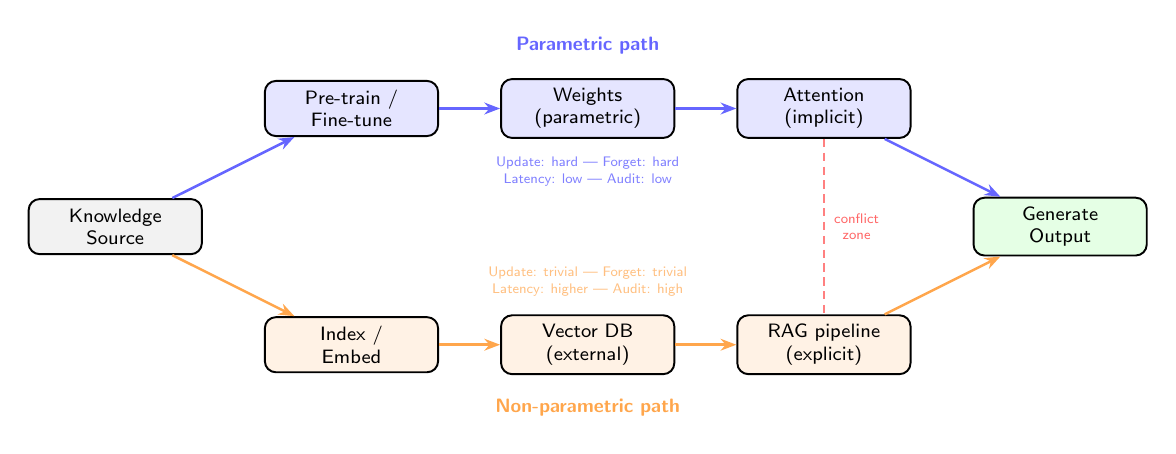
\begin{tikzpicture}[
  box/.style={draw, rounded corners=4pt, minimum width=2.2cm, minimum height=0.7cm, font=\sffamily\scriptsize, align=center, line width=0.7pt},
  parrow/.style={-{Stealth[length=2mm]}, line width=0.9pt, color=blue!60},
  nparrow/.style={-{Stealth[length=2mm]}, line width=0.9pt, color=orange!70},
  plabel/.style={font=\sffamily\scriptsize\bfseries, color=blue!60},
  nlabel/.style={font=\sffamily\scriptsize\bfseries, color=orange!70}
]

% --- Left: Knowledge source ---
\node[box, fill=gray!10] (src) at (0,0) {Knowledge\\Source};

% --- Parametric path (top) ---
\node[box, fill=blue!10] (ptrain) at (3, 1.5) {Pre-train /\\Fine-tune};
\node[box, fill=blue!10] (pstore) at (6, 1.5) {Weights\\(parametric)};
\node[box, fill=blue!10] (pret)   at (9, 1.5) {Attention\\(implicit)};

% --- Non-parametric path (bottom) ---
\node[box, fill=orange!10] (nindex) at (3, -1.5) {Index /\\Embed};
\node[box, fill=orange!10] (nstore) at (6, -1.5) {Vector DB\\(external)};
\node[box, fill=orange!10] (nret)   at (9, -1.5) {RAG pipeline\\(explicit)};

% --- Merge point ---
\node[box, fill=green!10] (gen) at (12, 0) {Generate\\Output};

% --- Parametric arrows ---
\draw[parrow] (src) -- (ptrain);
\draw[parrow] (ptrain) -- (pstore);
\draw[parrow] (pstore) -- (pret);
\draw[parrow] (pret) -- (gen);

% --- Non-parametric arrows ---
\draw[nparrow] (src) -- (nindex);
\draw[nparrow] (nindex) -- (nstore);
\draw[nparrow] (nstore) -- (nret);
\draw[nparrow] (nret) -- (gen);

% --- Conflict zone ---
\draw[densely dashed, red!50, line width=0.8pt] (pret) -- (nret) node[midway, right, font=\sffamily\tiny, text=red!60, align=center] {conflict\\zone};

% --- Path labels ---
\node[plabel] at (6, 2.3) {Parametric path};
\node[nlabel] at (6, -2.3) {Non-parametric path};

% --- Properties ---
\node[font=\sffamily\tiny, text=blue!50, align=center] at (6, 0.7) {Update: hard | Forget: hard\\Latency: low | Audit: low};
\node[font=\sffamily\tiny, text=orange!50, align=center] at (6, -0.7) {Update: trivial | Forget: trivial\\Latency: higher | Audit: high};

\end{tikzpicture}
\caption{Two paths through the knowledge lifecycle. The parametric path (top, blue) bakes knowledge into weights during training; it is fast at inference but hard to update or forget. The non-parametric path (bottom, orange) stores knowledge externally; it is easy to modify but depends on retrieval quality. When both paths are active, the ``conflict zone'' (dashed red) produces the knowledge conflict problem discussed in \S\ref{sec:update}.}
\label{fig:two_paths}
\end{figure}

\subsection{Parametric vs.\ Non-Parametric: A Unified View}

The single most important design decision in any LLM knowledge system is where to put the knowledge: in the weights or outside them. Figure~\ref{fig:two_paths} visualises the two paths, and Table~\ref{tab:parametric_comparison} lays out how this choice plays out across every lifecycle stage.

\begin{table}[t]
\centering
\caption{How the parametric/non-parametric choice affects each lifecycle stage.}
\label{tab:parametric_comparison}
\small
\begin{tabular}{@{}lll@{}}
\toprule
\textbf{Lifecycle Stage} & \textbf{Parametric} & \textbf{Non-Parametric} \\
\midrule
Acquisition & Pre-training, fine-tuning & Indexing documents \\
Storage & Distributed in weights & Explicit in databases \\
Retrieval & Attention (implicit) & Search pipeline (explicit) \\
Update & Knowledge editing (hard) & Database write (trivial) \\
Forgetting & Unlearning (hard) & Delete entry (trivial) \\
\midrule
Latency & Low (single forward pass) & Higher (retrieval + generation) \\
Auditability & Low (opaque weights) & High (traceable sources) \\
Scalability & Fixed at training time & Grows with corpus \\
\bottomrule
\end{tabular}
\end{table}

The pattern is consistent. Parametric storage is fast and tightly integrated with the model's reasoning, but opaque, rigid, and difficult to modify. Non-parametric storage is modular and transparent, but depends entirely on the retrieval pipeline's ability to surface the right knowledge at the right time. The most promising path forward is lifecycle-aware hybrid design: route stable, frequently accessed knowledge into the weights, and route dynamic, auditable, regulation-sensitive knowledge into external stores where it can be updated and deleted without touching the model.

\subsection{Scalability Across Lifecycle Stages}

Each lifecycle stage has its own scalability bottleneck. Pre-training costs now exceed \$100M for frontier models. Vector databases must handle billions of embeddings without degrading query latency. Knowledge editing methods break down after a few thousand edits. Unlearning must be verified across the model's entire output distribution, which is effectively infinite.

These bottlenecks interact. Training on more data creates a larger parametric store that is harder to edit and harder to unlearn from. Expanding a non-parametric store improves coverage but increases the candidate pool that the retriever must search through, raising the probability of returning irrelevant results. These inter-stage scaling effects are rarely studied, because researchers typically optimise for one stage at a time.

\subsection{Evaluation Methods and Benchmarks}

Every lifecycle stage has its own evaluation protocol, and none of them accounts for the others. RAG systems measure retrieval recall and end-to-end answer quality (RAGAS~\citep{es2024ragas}, Benchmarking RAG~\citep{chen2024benchmarking_rag}). Knowledge editing measures efficacy, specificity, and generalisation~\citep{yao2023editing_survey}. Unlearning measures whether the target knowledge can be extracted via membership inference attacks~\citep{maini2024tofu}. Agent memory systems are beginning to use multi-session benchmarks that test whether an agent can recall information from 50 conversations ago.

The gap is obvious. A system can score well on a RAG benchmark and a knowledge editing benchmark individually, while failing catastrophically when the two stages interact (e.g., when an edited fact is overridden by a stale retrieved passage). What the field needs is a lifecycle benchmark: a test suite that evaluates a sequence of operations (store, retrieve, update, verify the update, forget, verify the deletion) on the same set of facts. No such benchmark exists today.

\subsection{The Knowledge Consistency Problem}

The hardest cross-stage problem is consistency. As knowledge flows through the lifecycle, inconsistencies accumulate from at least four sources:

\begin{itemize}[leftmargin=*]
  \item \textbf{Temporal.} The weights reflect the training cutoff. The retrieved documents reflect the current date. The model may blend the two, producing an answer that is partly outdated and partly current.
  \item \textbf{Source-level.} Two retrieved documents may contradict each other. The model has no mechanism to determine which source is more reliable.
  \item \textbf{Edit-level.} An edit changes ``The capital of Country X is A'' to ``The capital of Country X is B,'' but leaves all related facts (e.g., ``A is the largest city in Country X'') unchanged. The model's knowledge is now internally contradictory.
  \item \textbf{Forgetting-level.} An unlearning operation removes a fact when asked directly, but the model can still reconstruct it from indirect cues. The fact is technically ``forgotten'' but practically recoverable.
\end{itemize}

Consistency is a lifecycle problem by definition. It cannot be fixed at any single stage. Fixing it would require a knowledge provenance system that tracks every fact through every stage: when it was acquired, where it is stored, how it has been retrieved, whether it has been updated, and whether it has been marked for deletion. Building such a system is a major open engineering and research challenge.

% ============================================================
\section{Open Problems and Future Directions}
\label{sec:open_problems}
% ============================================================

\subsection{Unified Benchmarks for the Full Lifecycle}

The field needs benchmarks that test \textit{sequences} of lifecycle operations, not individual stages. A lifecycle benchmark would work as follows: (1) the system ingests a corpus of facts, (2) it is tested on retrieval accuracy, (3) a subset of facts is updated, (4) the system is re-tested to verify that updates have propagated and that non-updated facts are unaffected, (5) a subset of facts is marked for deletion, and (6) the system is tested to verify that deleted facts are truly inaccessible, including through indirect queries. Each step is straightforward; the value is in chaining them together and measuring the cumulative error.

\subsection{End-to-End Differentiable Knowledge Systems}

Current RAG pipelines are modular but non-differentiable: the retriever and the generator are trained separately, and the boundary between them is a hard discrete selection of top-$k$ passages. Early work on joint training~\citep{guu2020realm, izacard2022atlas} showed that end-to-end optimisation improves both retrieval quality and generation quality. Extending this idea across the full lifecycle (jointly optimising acquisition, storage format, retrieval strategy, update mechanisms, and forgetting policies) is a long-term research goal. It would require differentiable approximations of inherently discrete operations like database insertion and deletion, which is technically challenging but not inconceivable given recent advances in differentiable data structures.

\subsection{Trustworthy Knowledge Management}

Deploying LLMs in medicine, law, and finance demands more than accuracy; it demands accountability. Three capabilities are needed. First, \textit{knowledge provenance}: every fact the system uses should carry metadata recording its source, its acquisition date, and its confidence level. Second, \textit{knowledge verification}: an independent check that stored and retrieved facts are consistent with ground truth. Third, \textit{knowledge auditing}: the ability for a regulator or end user to inspect what the model knows and how it came to know it. No production system today provides all three. The lifecycle framework makes clear that these capabilities must span all five stages; bolting provenance tracking onto the retrieval stage alone is insufficient if the fact was acquired during pre-training and later edited.

\subsection{Multi-Modal Knowledge Lifecycles}

This survey covers text. But LLMs are rapidly becoming multimodal, and each new modality brings its own lifecycle challenges. How should a model acquire and store visual knowledge (e.g., the layout of a building from a floor plan)? How should it retrieve cross-modal knowledge (e.g., answering a text question about an image)? How should it update visual knowledge when the physical world changes (e.g., a building is renovated)? These questions are natural extensions of the lifecycle framework and represent a largely open frontier.

\subsection{Knowledge Lifecycles for Multi-Agent Systems}

When multiple LLM agents collaborate on a task, knowledge management becomes a distributed systems problem. Agents must share knowledge without creating inconsistencies. They must coordinate updates so that one agent's edit does not conflict with another agent's cached version of the same fact. They must manage access control so that sensitive knowledge is available to authorised agents and hidden from others. The lifecycle framework suggests that each agent maintains its own local lifecycle while participating in a collective lifecycle at the system level. The distributed systems community has decades of experience with consistency, replication, and conflict resolution protocols; applying these ideas to multi-agent LLM systems is a promising and largely unexplored direction.

% ============================================================
\section{Conclusion}
\label{sec:conclusion}
% ============================================================

This survey has argued that the five subfields studying knowledge in LLMs (retrieval-augmented generation, knowledge editing, continual learning, context engineering, and agent memory) are best understood as stages of a single \textit{Knowledge Lifecycle}. We organised the literature into five stages (Acquisition, Storage, Retrieval, Update, Forgetting), reviewed each in detail, and identified cross-stage failure modes that no single-stage survey can detect.

Three findings stand out. First, the parametric/non-parametric storage choice is not a one-time design decision; it propagates through every subsequent stage, shaping what can be retrieved, how easily it can be updated, and how completely it can be forgotten. Second, the hardest open problems (knowledge conflicts, edit consistency, unlearning verification) live at the boundaries between stages, not within them. Third, the field lacks evaluation tools that test knowledge management end to end; building lifecycle benchmarks is both feasible and urgent.

As LLMs evolve from stateless responders into persistent, knowledge-managing agents, the lifecycle perspective will only grow in importance. The next generation of these systems will be judged not by how well they perform at any single stage, but by how coherently they manage the full lifecycle: acquiring knowledge where it is needed, storing it where it belongs, retrieving it when it matters, updating it as the world changes, and forgetting it when the law or common sense demands.

\bibliographystyle{plainnat}
\bibliography{references}

\end{document}
